Research on dynamical and hybrid systems has produced several methods
for verification and controller synthesis.
A common step in these methods is the reachability analysis of the system.
Reachability analysis is concerned with the  computation of the reach set
in  a way that can effectively meet requests like the following:
\begin{enumerate}
\item For a given target set and time, determine whether
the reach set and the target set have nonempty intersection.
\item For specified reachable state and time,
find a feasible initial condition and control that steers the system
from this initial condition to the given reachable state in given time.
\item Graphically display the projection of the reach set onto
any specified two- or three-dimensional subspace.
\end{enumerate}
Except for very specific classes of systems, exact computation of reach sets is
not possible, and approximation techniques are needed.
For controlled linear systems with convex bounds on the control
and initial conditions, the efficiency and accuracy of these techniques depend
on how they represent convex sets and how well they perform the operations
of unions, intersections, geometric (Minkowski) sums and differences
of convex sets.
Two basic objects are used as convex approximations:
polytopes of various types, including general polytopes, zonotopes,
parallelotopes, rectangular polytopes; and ellipsoids.

Reachability analysis for general polytopes is implemented in the
Multi Parametric Toolbox (MPT) for Matlab \cite{morari, mpt}.
The reach set at every time step is computed as the geometric sum
of two polytopes. The procedure consists in finding the vertices
of the resulting polytope and calculating their convex hull.
MPT's convex hull algorithm is based on the Double Description
method \cite{motzkin} and implemented in the CDD/CDD+ package \cite{cdd}.
Its complexity is $V^n$, where $V$ is the number of vertices and $n$ is the
state space dimension. Hence the use of MPT is practicable for low dimensional
systems. But even in low dimensional systems the number of vertices in
the reach set polytope can grow very large with the number
of time steps. For example, consider the  system,
\[ x_{k+1} = Ax_k + u_k ,\]
with $A=\left[\begin{array}{cc}
\cos 1 & -\sin 1\\
\sin 1 & \cos 1\end{array}\right]$,
$u_k \in \{u\in {\bf R}^2 ~|~ \|u\|_{\infty}\leq 1\}$, and
$x_0 \in \{x\in {\bf R}^2 ~|~ \|x\|_{\infty}\leq 1\}$. Starting with a
rectangular initial set, the number of vertices of the reach set polytope
is $4k + 4$ at the $k$th step.

In $d/dt$ \cite{ddt},
the reach set is approximated by unions of rectangular polytopes \cite{maler}.
\begin{figure}[htbp]
\centerline{
\includegraphics[width=6.5 cm, height=8 cm]{ddt.eps}}
\caption{Reach set approximation by union of rectangles.
Source: adapted from \cite{maler}.}
\label{ddtfig}
\end{figure}
The algorithm works as follows. First, given the set of initial conditions
defined as a polytope, the evolution in time of the polytope's extreme points
is computed (figure \ref{ddtfig}(a)).
$R(t_1)$ in figure \ref{ddtfig}(a) is the
reach set of the system at time $t_1$, and $R[t_0, t_1]$ is the set of all
points that can be reached during $[t_0, t_1]$. Second, the
algorithm computes the convex hull of vertices of both, the initial polytope
and $R(t_1)$ (figure \ref{ddtfig}(b)).
The resulting polytope is then bloated to include
all the reachable states in $[t_0,t_1]$
(figure \ref{ddtfig}(c)). Finally, this overapproximating polytope is in its
turn overapproximated by the union of rectangles (figure \ref{ddtfig}(d)).
The same procedure is repeated for the next time interval $[t_1,t_2]$, and
the union of both rectangular approximations is taken
(figure \ref{ddtfig}(e,f)), and so on.
Rectangular polytopes are easy to represent and the number
of facets grows linearly with dimension, but a large number of rectangles
must be used to assure the approximation is not overly conservative.
Besides, the important part of this method is again the convex hull
calculation whose implementation relies on the same CDD/CDD+
library. This limits the dimension of the system and time interval
for which it is feasible to calculate the reach set.

Polytopes can give arbitrarily close approximations to any convex set,
but the number of vertices can grow prohibitively large and,
as shown in \cite{avis}, the computation of a polytope by its convex hull
becomes intractable for large number of vertices in high dimensions.

The method of zonotopes for approximation of reach sets
\cite{girard, leguernic, matisse} uses a special class of polytopes
(see \cite{zonotool}) of the form,
\[ Z=\{x \in {\bf R}^n ~|~
x=c+\sum_{i=1}^p\alpha_ig_i,~ -1\leq\alpha_i\leq1\}, \]
wherein $c$ and $g_1, ..., g_p$ are vectors in ${\bf R}^n$. Thus, a
zonotope $Z$ is  represented by its center $c$ and `generator' vectors
$g_1, ..., g_p$. The value $p/n$ is called the order of the zonotope.
The main benefit of zonotopes over general polytopes is that a symmetric
polytope can be represented more compactly than a general polytope.
The geometric sum of two zonotopes is a zonotope:
\[ Z(c_1, G_1)\oplus Z(c_2, G_2) = Z(c_1+c_2, [G_1 ~ G_2]), \]
wherein $G_1$ and $G_2$ are matrices whose columns are generator vectors,
and $[G_1 ~ G_2]$ is their concatenation. Thus, in the reach set computation,
the order of the zonotope increases by $p/n$ with every time step.
This difficulty can be averted by limiting the number of generator vectors,
and overapproximating zonotopes whose number of generator vectors exceeds
the limit by lower order zonotopes.
The benefits of the compact zonotype representation, however, appear
to diminish because in order to plot them or check if they
intersect with given objects and compute those intersections,
these operations are performed after converting zonotopes to polytopes.

CheckMate \cite{checkmate} is a Matlab toolbox that can evaluate specifications
for trajectories starting from the set of initial (continuous) states
corresponding to the parameter values at the vertices of the parameter set.
This provides preliminary insight into whether the specifications will be true
for all parameter values.
The method of oriented rectangluar polytopes for external approximation
of reach sets is introduced in \cite{krogh}.
The basic idea is to construct an oriented
rectangular hull of the reach set for every time step, whose orientation is
determined by the singular value decomposition of the sample covariance matrix
for the states reachable from the vertices of the initial polytope.
The limitation of CheckMate and the method of oriented rectangles is
that only autonomous (i.e. uncontrolled) systems, or  systems with fixed
input are allowed, and only an external approximation of the reach set
is provided.

All the methods described so far employ the notion of time step,
and calculate the reach set or its approximation at each time step.
This approach can be used only with discrete-time systems.
By contrast, the analytic methods which we are about to discuss,
provide a formula or differential equation describing the (continuous)
time evolution of the reach set or its approximation.

The level set method \cite{mitchell,levelset} deals with general
nonlinear controlled systems and gives exact representation of
their reach sets, but requires solving the HJB equation and finding
the set of states that belong to sub-zero level set of the value function.
The method \cite{levelset} is impractical for systems of dimension higher
than three.

Requiem \cite{requiem} is a Mathematica notebook which, given a linear system,
the set of initial conditions and control bounds, symbolically computes
the exact reach set, using the experimental quantifier elimination package.
Quantifier elimination is the removal of all quantifiers (the universal
quantifier $\forall$ and the existential quantifier $\exists$) from a quantified
system. Each quantified formula is substituted with quantifier-free expression
with operations $+$, $\times$, $=$ and $<$. For example, consider the
discrete-time system
\[ x_{k+1} = Ax_k + Bu_k \]
with $A=\left[\begin{array}{cc}
0 & 1\\
0 & 0\end{array}\right]$ and $B=\left[\begin{array}{c}
0\\
1\end{array}\right]$.  For initial conditions
$x_0\in\{x\in {\bf R}^2 ~|~ \|x\|_{\infty} \leq 1\}$ and controls
$u_k\in\{u\in {\bf R} ~|~ -1\leq u\leq1\}$, the reach set for  $k\geq0$
is given by the quantified formula
\[\{ x\in{\bf R}^2 ~|~ \exists x_0, ~~ \exists k\geq 0, ~~
\exists u_i, ~ 0\leq i\leq k: ~~
x = A^kx_0+\sum_{i=0}^{k-1}A^{k-i-1}Bu_i \}, \]
which is equivalent to the quantifier-free expression
\[ -1\leq[1 ~~ 0]x\leq1 ~ \wedge ~ -1\leq[0 ~~ 1]x\leq1. \]
It is proved in \cite{yovine} that for continuous-time systems,
$\dot{x}(t) = Ax(t) + Bu(t)$, if $A$ is constant and nilpotent or
is diagonalizable with rational real or purely imaginary eigenvalues,
and with suitable restrictions on the control and initial conditions,
the quantifier elimination package returns a quantifier free formula
describing the reach set. Quantifier elimination has limited applicability.

The reach set approximation via parallelotopes \cite{kostousova} employs
the idea of parametrization described in \cite{kurvar} for ellipsoids.
The reach set is represented as the intersection of tight external,
and the union of tight internal, parallelotopes.
The evolution equations for the centers and
orientation matrices of both external and internal parallelotopes are
provided. This method also finds controls that can drive the system to
the boundary points of the reach set, similarly to \cite{varaiya}
and \cite{kurvar}. It works for general linear systems.  The
computation to solve the evolution equation for tight approximating
parallelotopes, however, is more involved than that for ellipsoids,
and for discrete-time systems this method does not deal with singular state
transition matrices.

{\it Ellipsoidal Toolbox} (ET) implements in MATLAB
the ellipsoidal calculus \cite{kurvalyi}
and its application to the reachability analysis of continuous-time
\cite{kurvar}, discrete-time \cite{pvak}, possibly time-varying linear systems,
and linear systems with disturbances \cite{kurvar2},
for which ET calculates both open-loop and close-loop reach sets.
The ellipsoidal calculus provides the following benefits:
\begin{itemize}
\item The complexity of the
ellipsoidal representation is quadratic in the dimension of
the state space, and linear in the number of time steps.
\item It is possible to exactly represent the reach set of
linear system through both external and internal ellipsoids.
\item It is possible to single out individual external and internal
approximating ellipsoids that are optimal to some given criterion
(e.g. trace, volume, diameter), or combination of such criteria.
\item We obtain simple analytical expressions for the control
that steers the state to a desired target.
\end{itemize}
\todo[inline]{Updated this list}
The report is organized as follows.
\newline
Chapter 2 describes the operations of the
ellipsoidal calculus: affine transformation, geometric sum,
geometric difference, intersections with
hyperplane, ellipsoid, halfspace and polytope, calculation of maximum ellipsoid,
calculation of minimum ellipsoid.
\newline
Chapter 3 presents the reachability problem and ellipsoidal methods for
the reach set approximation.
\newline
Chapter 4 contains {\it Ellipsoidal Toolbox} installation and quick start
instructions, and lists the software packages used by the toolbox.
\newline
Chapter 5 describes structures and objects implemented and used in toolbox.
Also it describes the implementation of methods from chapters 2 and 3
and visualization routines.
\newline
Chapter 6 describes structures and objects implemented and
used in the toolbox.
\newline
Chapter 6 gives examples of how to use the toolbox.
\newline
Chapter 7 collects some conclusions and plans for future toolbox development.
\newline
The functions provided by the toolbox together with their descriptions
are listed in appendix A.
